\documentclass[11pt]{article}

\usepackage{extras} % Se extras.sty

\begin{document}
\begin{titlepage}
\begin{center}

{\Large\bfseries TSEA56 - Kandidatprojekt i elektronik \\ LIPS Designspecifikation}

\vspace{5em}

Version 0.1

\vspace{5em}
Grupp 4 \\
\begin{tabular}{rl}
Hynén Ulfsjöö, Olle&\verb+ollul666+
\\
Wasteson, Emil&\verb+emiwa068+
\\
Tronje, Elena&\verb+eletr654+
\\
Gustafsson, Lovisa&\verb+lovgu777+
\\
Inge, Zimon&\verb+zimin415+
\\
Strömberg, Isak&\verb+isast763+
\\
\end{tabular}

\vspace{5em}
\today

\vspace{16em}
Status
\begin{longtable}{|l|l|l|} \hline

Granskad & - & - \\ \hline
Godkänd & - & - \\ \hline
 
\end{longtable}

\end{center}
\end{titlepage}

\pagebreak
\begin{center}

\section*{PROJEKTIDENTITET}
2016/VT, Undsättningsrobot Gr. 4

Linköpings tekniska högskola, ISY
\vspace{5em}
%\begin{center}

\begin{tabular}{|l|l|l|l|} \hline
\textbf{Namn} & \textbf{Ansvar} & \textbf{Telefon} & \textbf{E-post}  \\ \hline 
Isak Strömberg (IS) & Projektledare & 073-980 38 50 & isast763@student.liu.se \\ \hline
Olle Hynén Ulfsjöö (OHU)& Dokumentansvarig & 070-072 91 84 & ollul666@student.liu.se \\ \hline
Emil Wasteson (EW) & Hårdvaruansvarig & 076-836 61 66 & emiwa068@student.liu.se \\ \hline
Elena Tronje (ET) & Mjukvaruansvarig & 072-276 92 93 & eletr654@student.liu.se \\ \hline
Zimon Inge (ZI)& Testansvarig & 070-171 35 18 & zimin415@student.liu.se \\ \hline
Lovisa Gustafsson (LG) & Leveransansvarig & 070-210 32 53 & lovgu777@student.liu.se \\ \hline
\end{tabular}

%\end{center}

E-postlista för hela gruppen: isast763@student.liu.se

\vspace{5em}
Kund: ISY, Linköpings universitet \\
tel: 013-28 10 00, fax: 013-13 92 82 \\
Kontaktperson hos kund: Mattias Krysander \\
tel: 013-28 21 98, e-post: matkr@isy.liu.se \\

\vspace{5em}
Kursansvarig:  Tomas Svensson\\
tel: 013-28 13 68, e-post: tomass@isy.liu.se \\
Handledare: Peter Johansson \\
tel: 013-28 13 45, e-post: peter.a.johansson@liu.se
\end{center}
\pagebreak

\tableofcontents

\pagebreak

\section*{Dokumenthistorik}
\begin{table}[h]
\begin{tabular}{|l|l|l|l|l|} \hline

\textbf{Version} & \textbf{Datum} & \textbf{Utförda förändringar} & \textbf{Utförda av} & \textbf{Granskad} \\ \hline
0.1 & - &  Första utkastet & Grupp 4 & - \\ \hline
\end{tabular}
\end{table}

\pagebreak
\pagenumbering{arabic}

\begin{flushleft}
\section{Inledning}
\lipsum

\subsection{Det totala systemet}
\lipsum

\subsection{Sensorer}
\lipsum

\subsection{Ställdon}
\lipsum

\pagebreak
\section{Delmodul 1 - Huvudmodul}
\lipsum

\subsection{Detaljerad beskrivning}
\lipsum

\subsection{Hårdvara}
\lipsum

\subsection{Mjukvara}
\lipsum

\pagebreak
\section{Delmodul 2 - Sensormodul}
\lipsum

\subsection{Detaljerad beskrivning}
\lipsum

\subsection{Hårdvara}
\lipsum

\subsection{Mjukvara}
\lipsum

\pagebreak
\section{Delmodul 3 - Styrmodul}
\lipsum
%Styrmodulen tar emot kommandon från huvudmodulen och verkställer dessa. Det är antingen styrning av chassits motorer för att få roboten att röra på sig, rotera det eventuella lasersensortornet eller att styra gripklon. Kommunikationen sker genom I2C-bussen. Styrmodulen har även LCD-displayer kopplade till sig för att kunna skriva ut valda sensorvärden.



%För att skriva ut sensordata på display används den alphanumeriska LCD-displayen LCD JM162A. Den har totalt 16 pinnar, där 8 stycken är databitar, 3 stycken för konfiguration (inställning av funktion) och resterande är referenssignaler och strömtillförsel.

%Gripklon ska kunna öppnas och stängas på kommando från huvudmodulen.

\subsection{Detaljerad beskrivning}
Nedan följer en beskrivning av vilka styrkommandon styrmodulen ska kunna ta emot, hur kommunikationsprotokollet ser ut, hur regleringen ska ske samt lite övrig fakta kring modulen.

\subsubsection{Styrkommandon}\label{Styrkommandon}
Styrmodulen tar emot kommandon från huvudmodulen och verkställer dessa. Följande kommandon kommer kunna skickas: \textit{reglering av/på, gripklo öppna/stäng, fram/bak, sväng höger/vänster, rotera höger/vänster och stopp}. Kommandot \textit{reglering av/på} ställer in styrmodulen för manuell eller autonom körning, vilket påverkar tolkningen av det data som skickas från huvudmodulen.

Tillsammans med kommandona för rörelse skickas även ett tal som, beroende på om reglering är aktiverad eller inte, anger en sträcka/vinkel för förflyttningen eller med vilken hastighet (i procent av maxhastighet) förflyttningen ska utföras. Ett kommando kan exempelvis se ut såhär: \textit{fram 80}, varpå roboten antingen kör framåt 80 cm eller med 80\% av maxhastighet, beroende på om regleringen är aktiverad eller inte. Modulen kommer vara designad så att ett körkommando gäller tills dess att ett nytt kommando skickas, varför även kommandot för \textit{stopp} är nödvändigt.

Eftersom kommandona till styrmodulen skickas på den form som visats ovan kommer all reglering behöva ske i styrmodulen. Därför kommer även mätdata att tas emot från huvudmodulen. Beroende på vilken typ av förflyttning roboten utför så kommer följande sensorvärden att skickas från huvudmodulen:
\begin{itemize}
	\item fram/bak - avstånd till vägg fram och på sidorna.
	\item sväng höger/vänster - inga (kommandot används enbart vid manuell styrning och behöver således inte regleras).
	\item rotera höger/vänster - vinkel och vinkelhastighet.
\end{itemize}
Dessa sensorvärden kommer skickas med en frekvens av \textcolor{red}{x} Hz förutsatt att reglering är aktiverad, dvs vid autonom styrning av roboten.

\subsubsection{Kommunikationsprotokoll}
Följande protokoll används för att skicka data till styrmodulen:
\documentclass[crop,tikz]{standalone}
\usepackage{tikz}
\usetikzlibrary{calc}
\usetikzlibrary{positioning}
\begin{document}
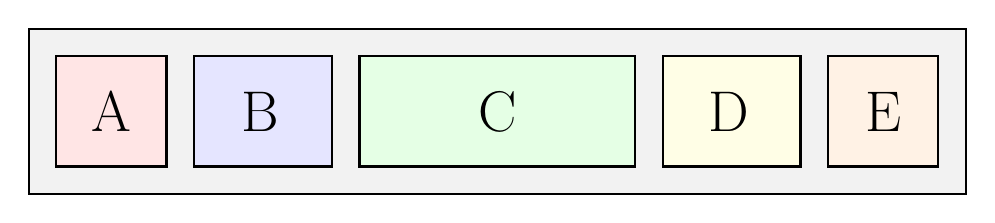
\begin{tikzpicture}[scale=0.07,rotate=0]
		
	%Frame
	\draw[thick, draw=black, fill=gray!10] (0,0) rectangle (170,30);

	%Segments
	%A
	\draw[thick, draw=black, fill=red!10] (5,5) rectangle (25,25);
	\node at (15,15) {\huge A};

	%B
	\draw[thick, draw=black, fill=blue!10] (30,5) rectangle (55,25);
	\node at (42,15) {\huge B};
	
	%C
	\draw[thick, draw=black, fill=green!10] (60,5) rectangle (110,25);
	\node at (85,15) {\huge C};

	%D
	\draw[thick, draw=black, fill=yellow!10] (115,5) rectangle (140,25);
	\node at (127,15) {\huge D};

	%E
	\draw[thick, draw=black, fill=orange!10] (145,5) rectangle (165,25);
	\node at (155,15) {\huge E};
	
\end{tikzpicture}
\end{document}

Där respektive segment motsvarar följande: 
\begin{itemize}
	\item A (Bit x-y) - Startbit
	\item B (Bit x-y) - Definierar om ett körkommando eller ett sensorvärde skickas.
	\item C (Bit x-y) - Definierar vilket kommando eller vilken typ av värde som skickas.
	\item D (Bit x-y) - Hastighet (om körkommando och inte reglering), sträcka/vinkel (om körkommande och reglering) eller värde (om sensorvärde).
	\item E (Bit x-y) - Slutbit
\end{itemize}

\subsubsection{Reglering}
Vid manuell styrning av roboten sker ingen reglering. Detta för att användaren ska få ohämmad kontroll över roboten och förväntas sköta ``regleringen'' manuellt. Vid autonom styrning kommer dock alla förflyttningar behöva regleras. Som nämnt i avsnitt \ref{Styrkommandon} kommer huvudmodulen skicka relevanta sensorvärden vid autonom körning. Beroende på vilket styrkommando som skickats väljer styrmodulen sedan en styrmod och reglerar rörelsen. De olika styrmoderna och hur deras reglering sker finns beskrivet mer ingående i Appendix \textcolor{red}{x}.

\subsubsection{Övrigt}
Plattformen som roboten byggs på har färdiga kretsar för att styra chassits hjul. Hjulen kan styras parvis (höger och vänster) genom att sätta en bit för att bestämma rotationsriktningen och sedan skicka en PWM-signal för att bestämma rotationshastigheten. Roboten styrs alltså differentiellt, dvs genom olika hastighet på höger och vänster sida.

Roboten ska även vara utrustad med en gripklo, för att kunna greppa de förnödenheter som ka transporteras. Klons aktiva del består av ett servo av typen \verb+RG-180+ som styrs med en PWM-signal.

Det ska även finnas en alphanumerisk LCD-display, av typen \verb+LCD JM162A+, på roboten, som används för att visa relevanta sensorvärden vid reglering. Den har totalt 16 pinnar, varav åtta är databitar, tre används för konfiguration och resterane är referensignaler och strömtillförsel.

\subsection{Hårdvara}
Styrmodulen kommer kräva följande hårdvara:
\begin{itemize}
	\item ATmega16
	\item Robotplattform (Terminator)
	\item Gripklo %Specificera senare
\end{itemize}

\subsection{Mjukvara}
\lipsum

\pagebreak
\section{Delmodul 4 - Datormodul}
\lipsum

\subsection{Detaljerad beskrivning}
\lipsum

\subsection{Hårdvara}
Datormodulen kräver en dator kompatibel med Java.

\subsection{Mjukvara}
\lipsum

\pagebreak
\section{Intermodulär kommunikation}
\lipsum

\subsection{I\textsuperscript{2}C-buss}
\lipsum

\subsection{Bluetooth\textsuperscript{\circledR}-kommunikation}
\lipsum

\pagebreak
\section{Implementering}
\lipsum

\end{flushleft}

\end{document}